\documentclass[paper=a4paper,jafontsize=9pt,head_space=15mm,gutter=20mm,
twocolumn,number_of_lines=49, line_length=26zw]{myuarticle}

\begin{document}

\title{{\Large\bfseries\gtfamily 環境情報のセンシングを用いた他者の環境評価を表現するロボットシステム}}
\author{\\\ 22120165 中村龍造 \\(指導教員 : 佐藤宏樹)\\ \\}
\date{}
\maketitle

\section*{研究概要}

\begin{figure*}[b]
  \begin{center}
    \begin{minipage}[b]{0.23\textwidth}
      \centering
      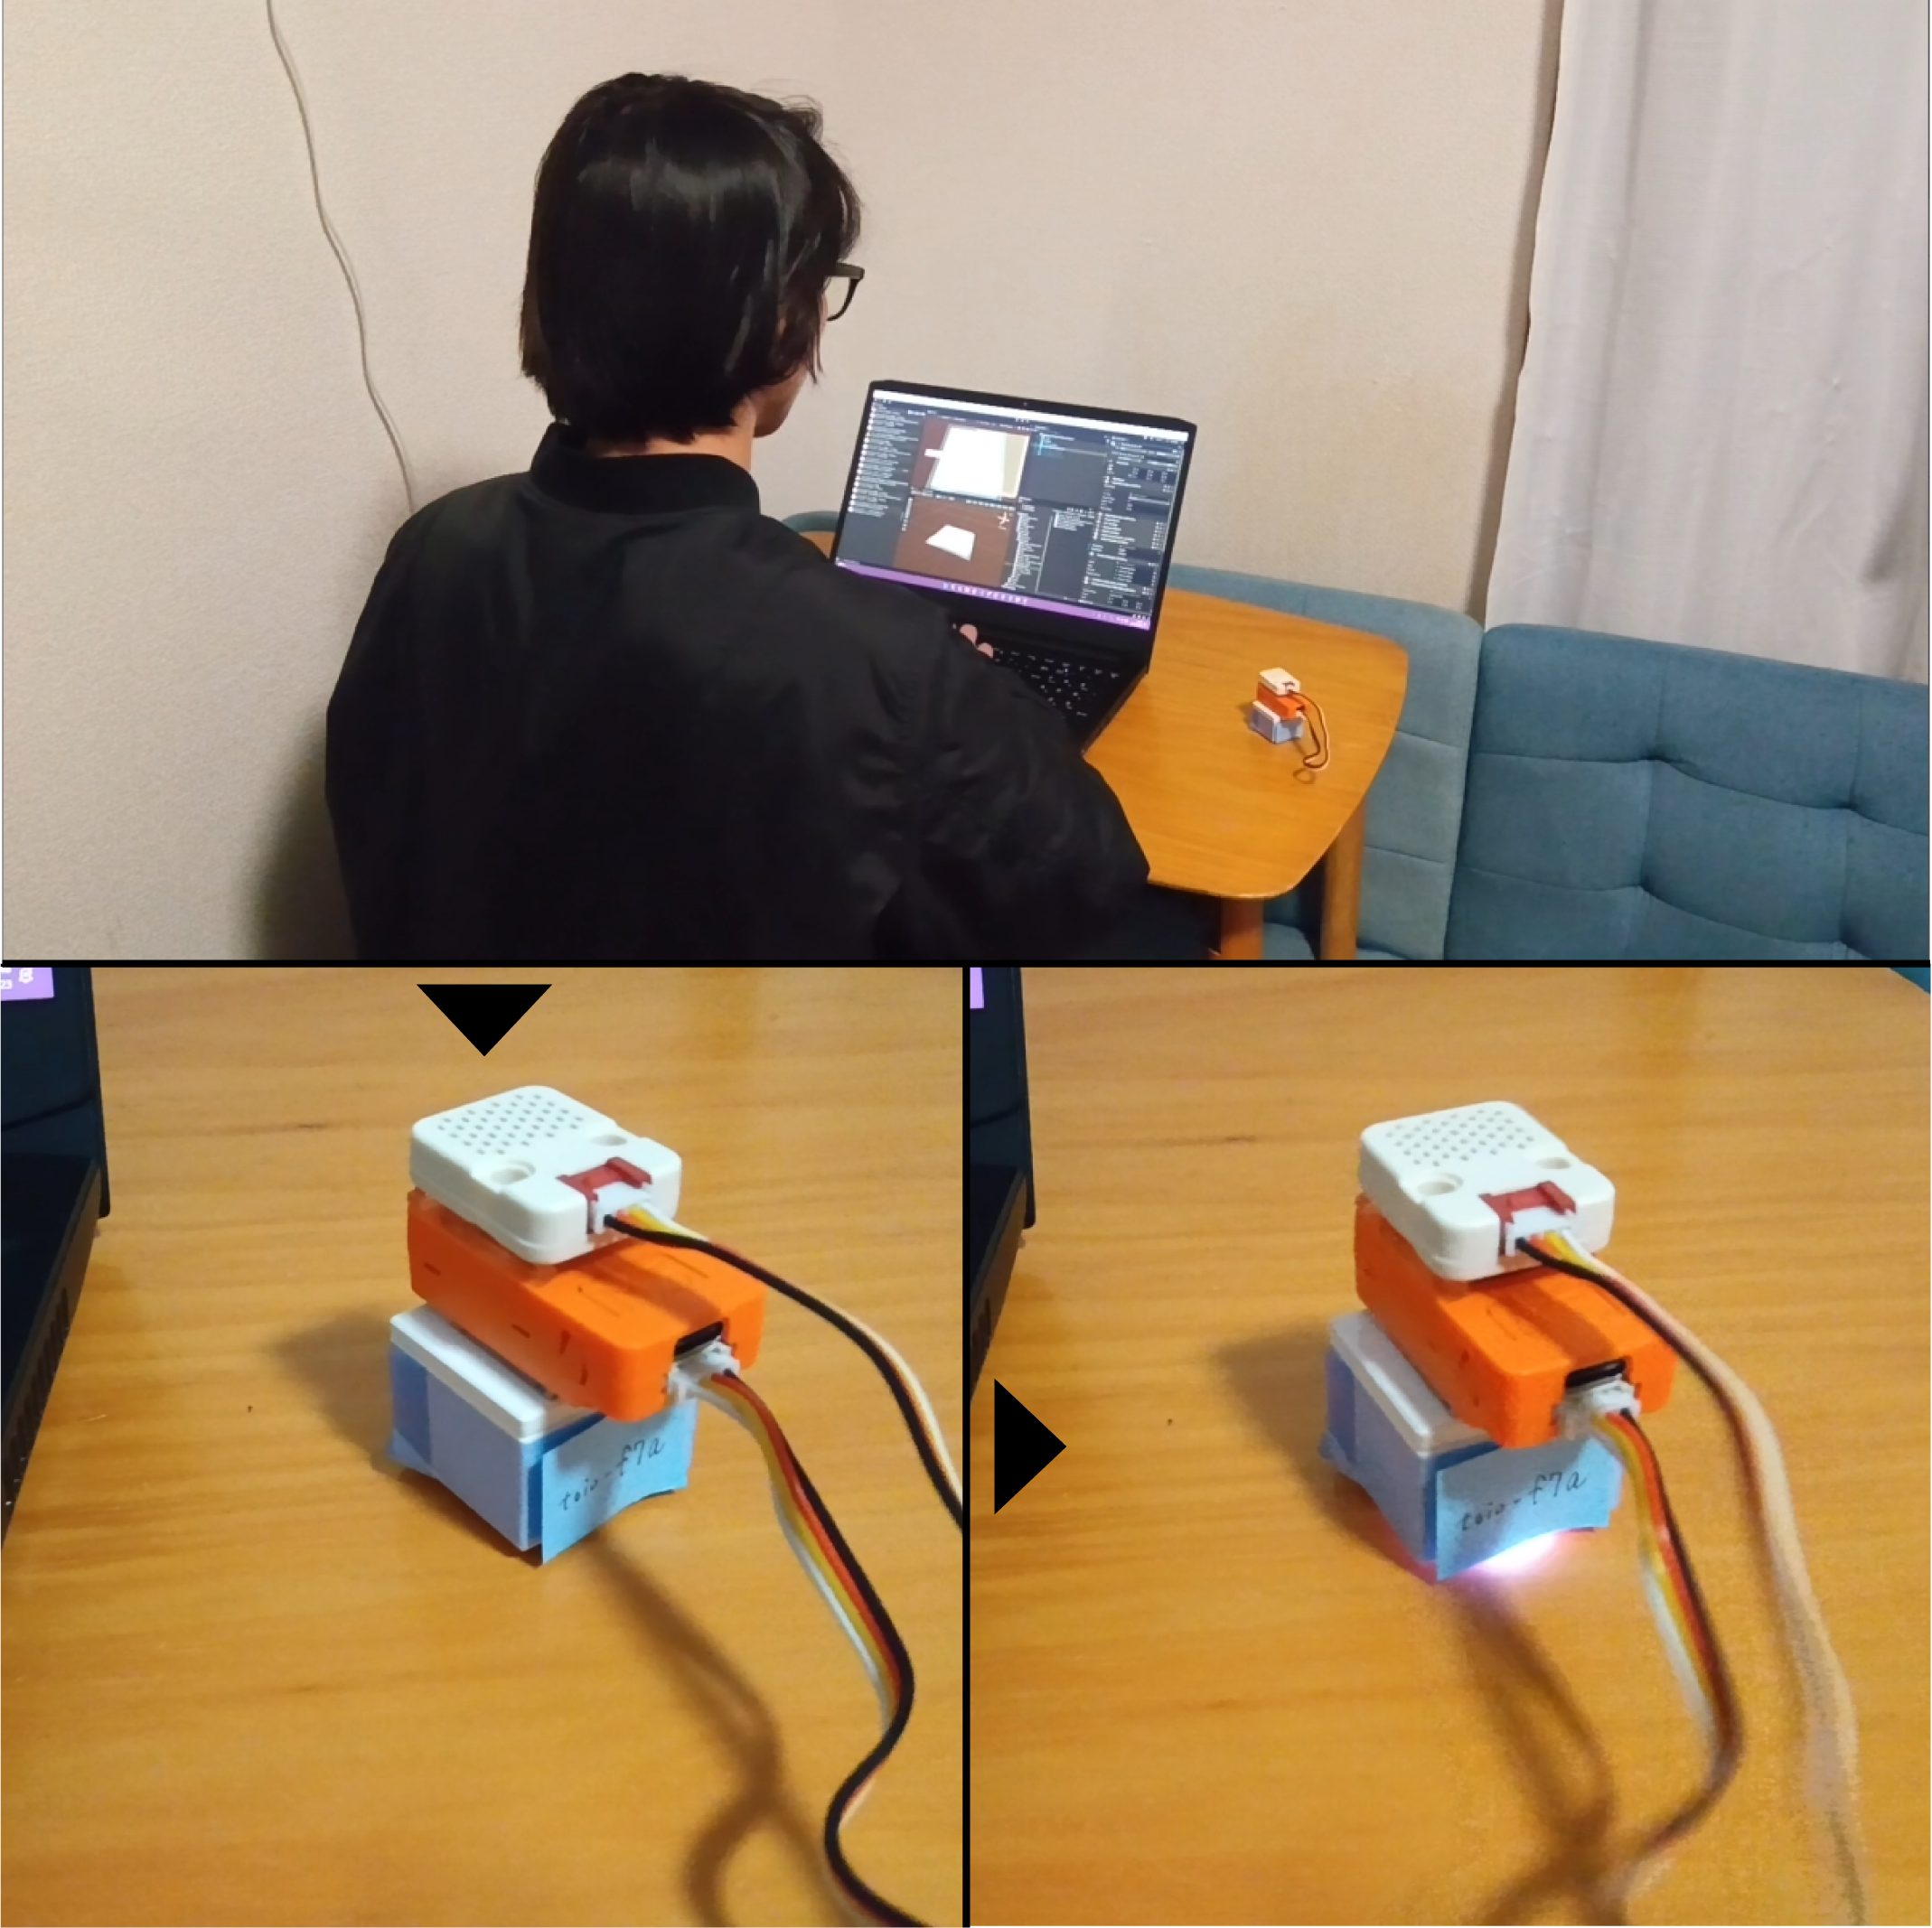
\includegraphics[keepaspectratio, scale=0.1]{resources/human.png}
      \caption{人間の気温評価}
    \end{minipage}
    \begin{minipage}[b]{0.23\textwidth}
      \centering
      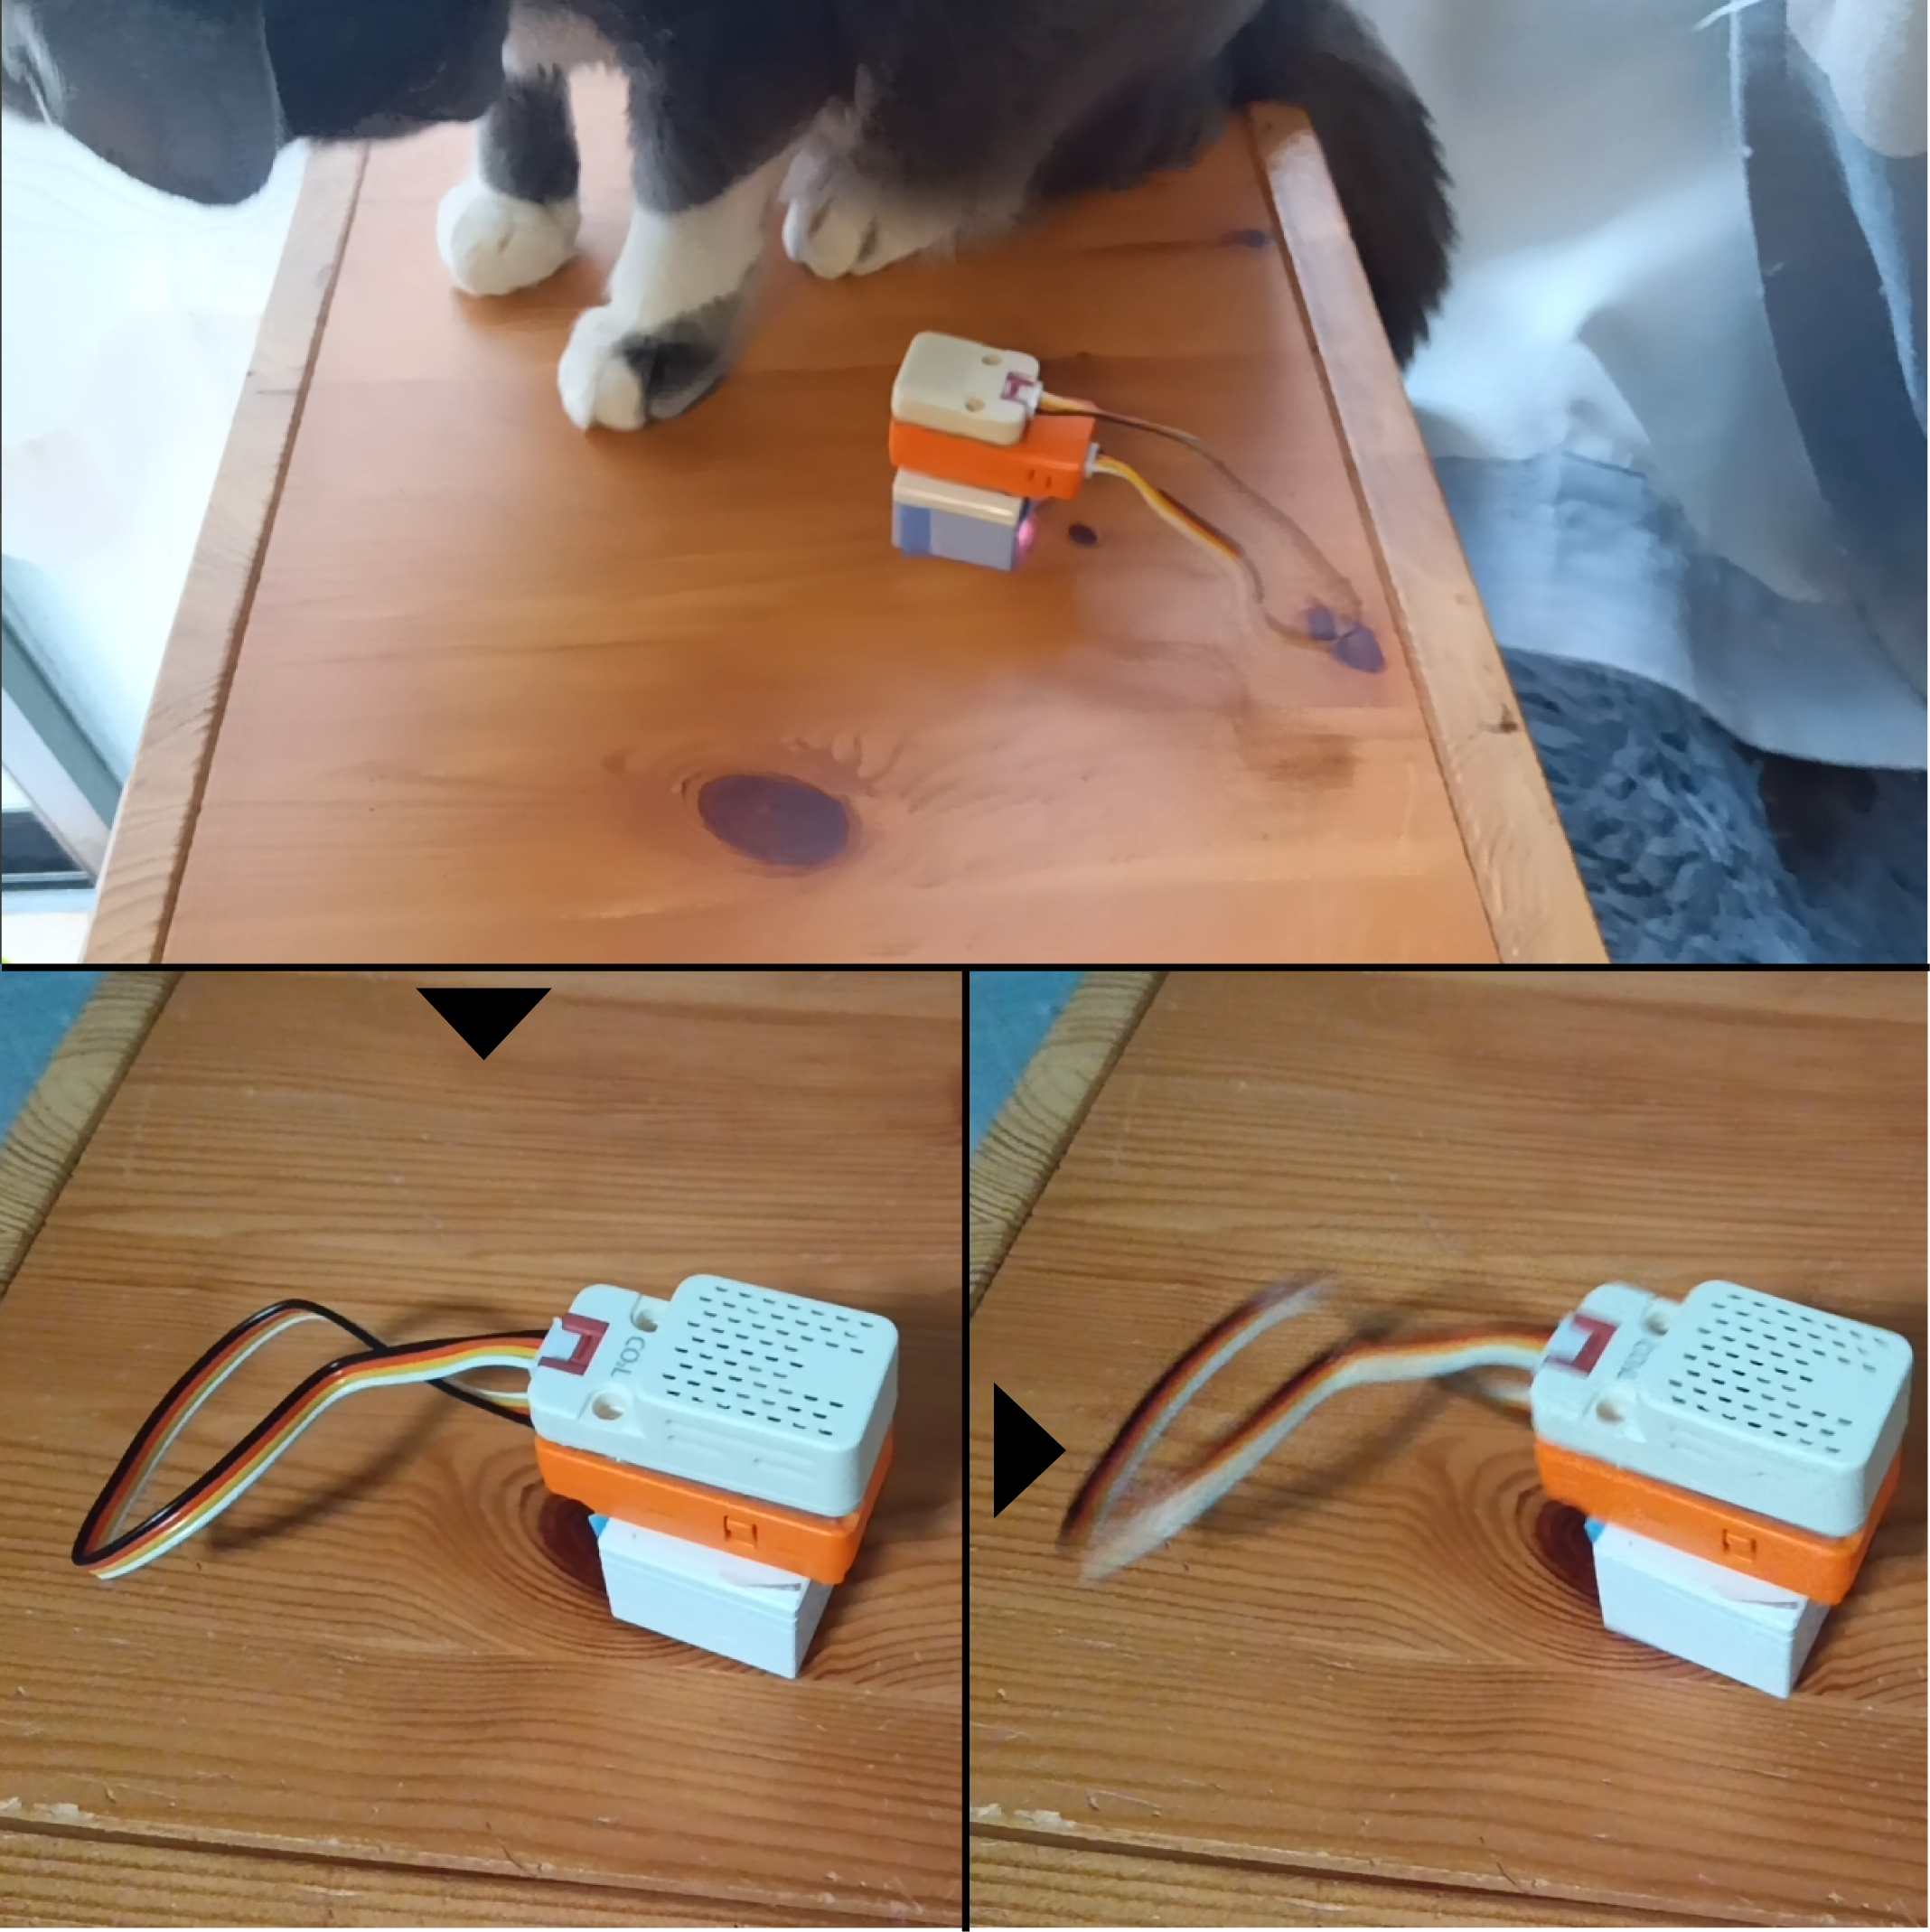
\includegraphics[keepaspectratio, scale=0.1]{resources/cat.png}
      \caption{猫の気温評価}
    \end{minipage}
    \begin{minipage}[b]{0.23\textwidth}
      \centering
      \includegraphics[keepaspectratio, scale=0.1]{resources/banana.png}
      \caption{バナナの環境評価}
    \end{minipage}
    \begin{minipage}[b]{0.23\textwidth}
      \centering
      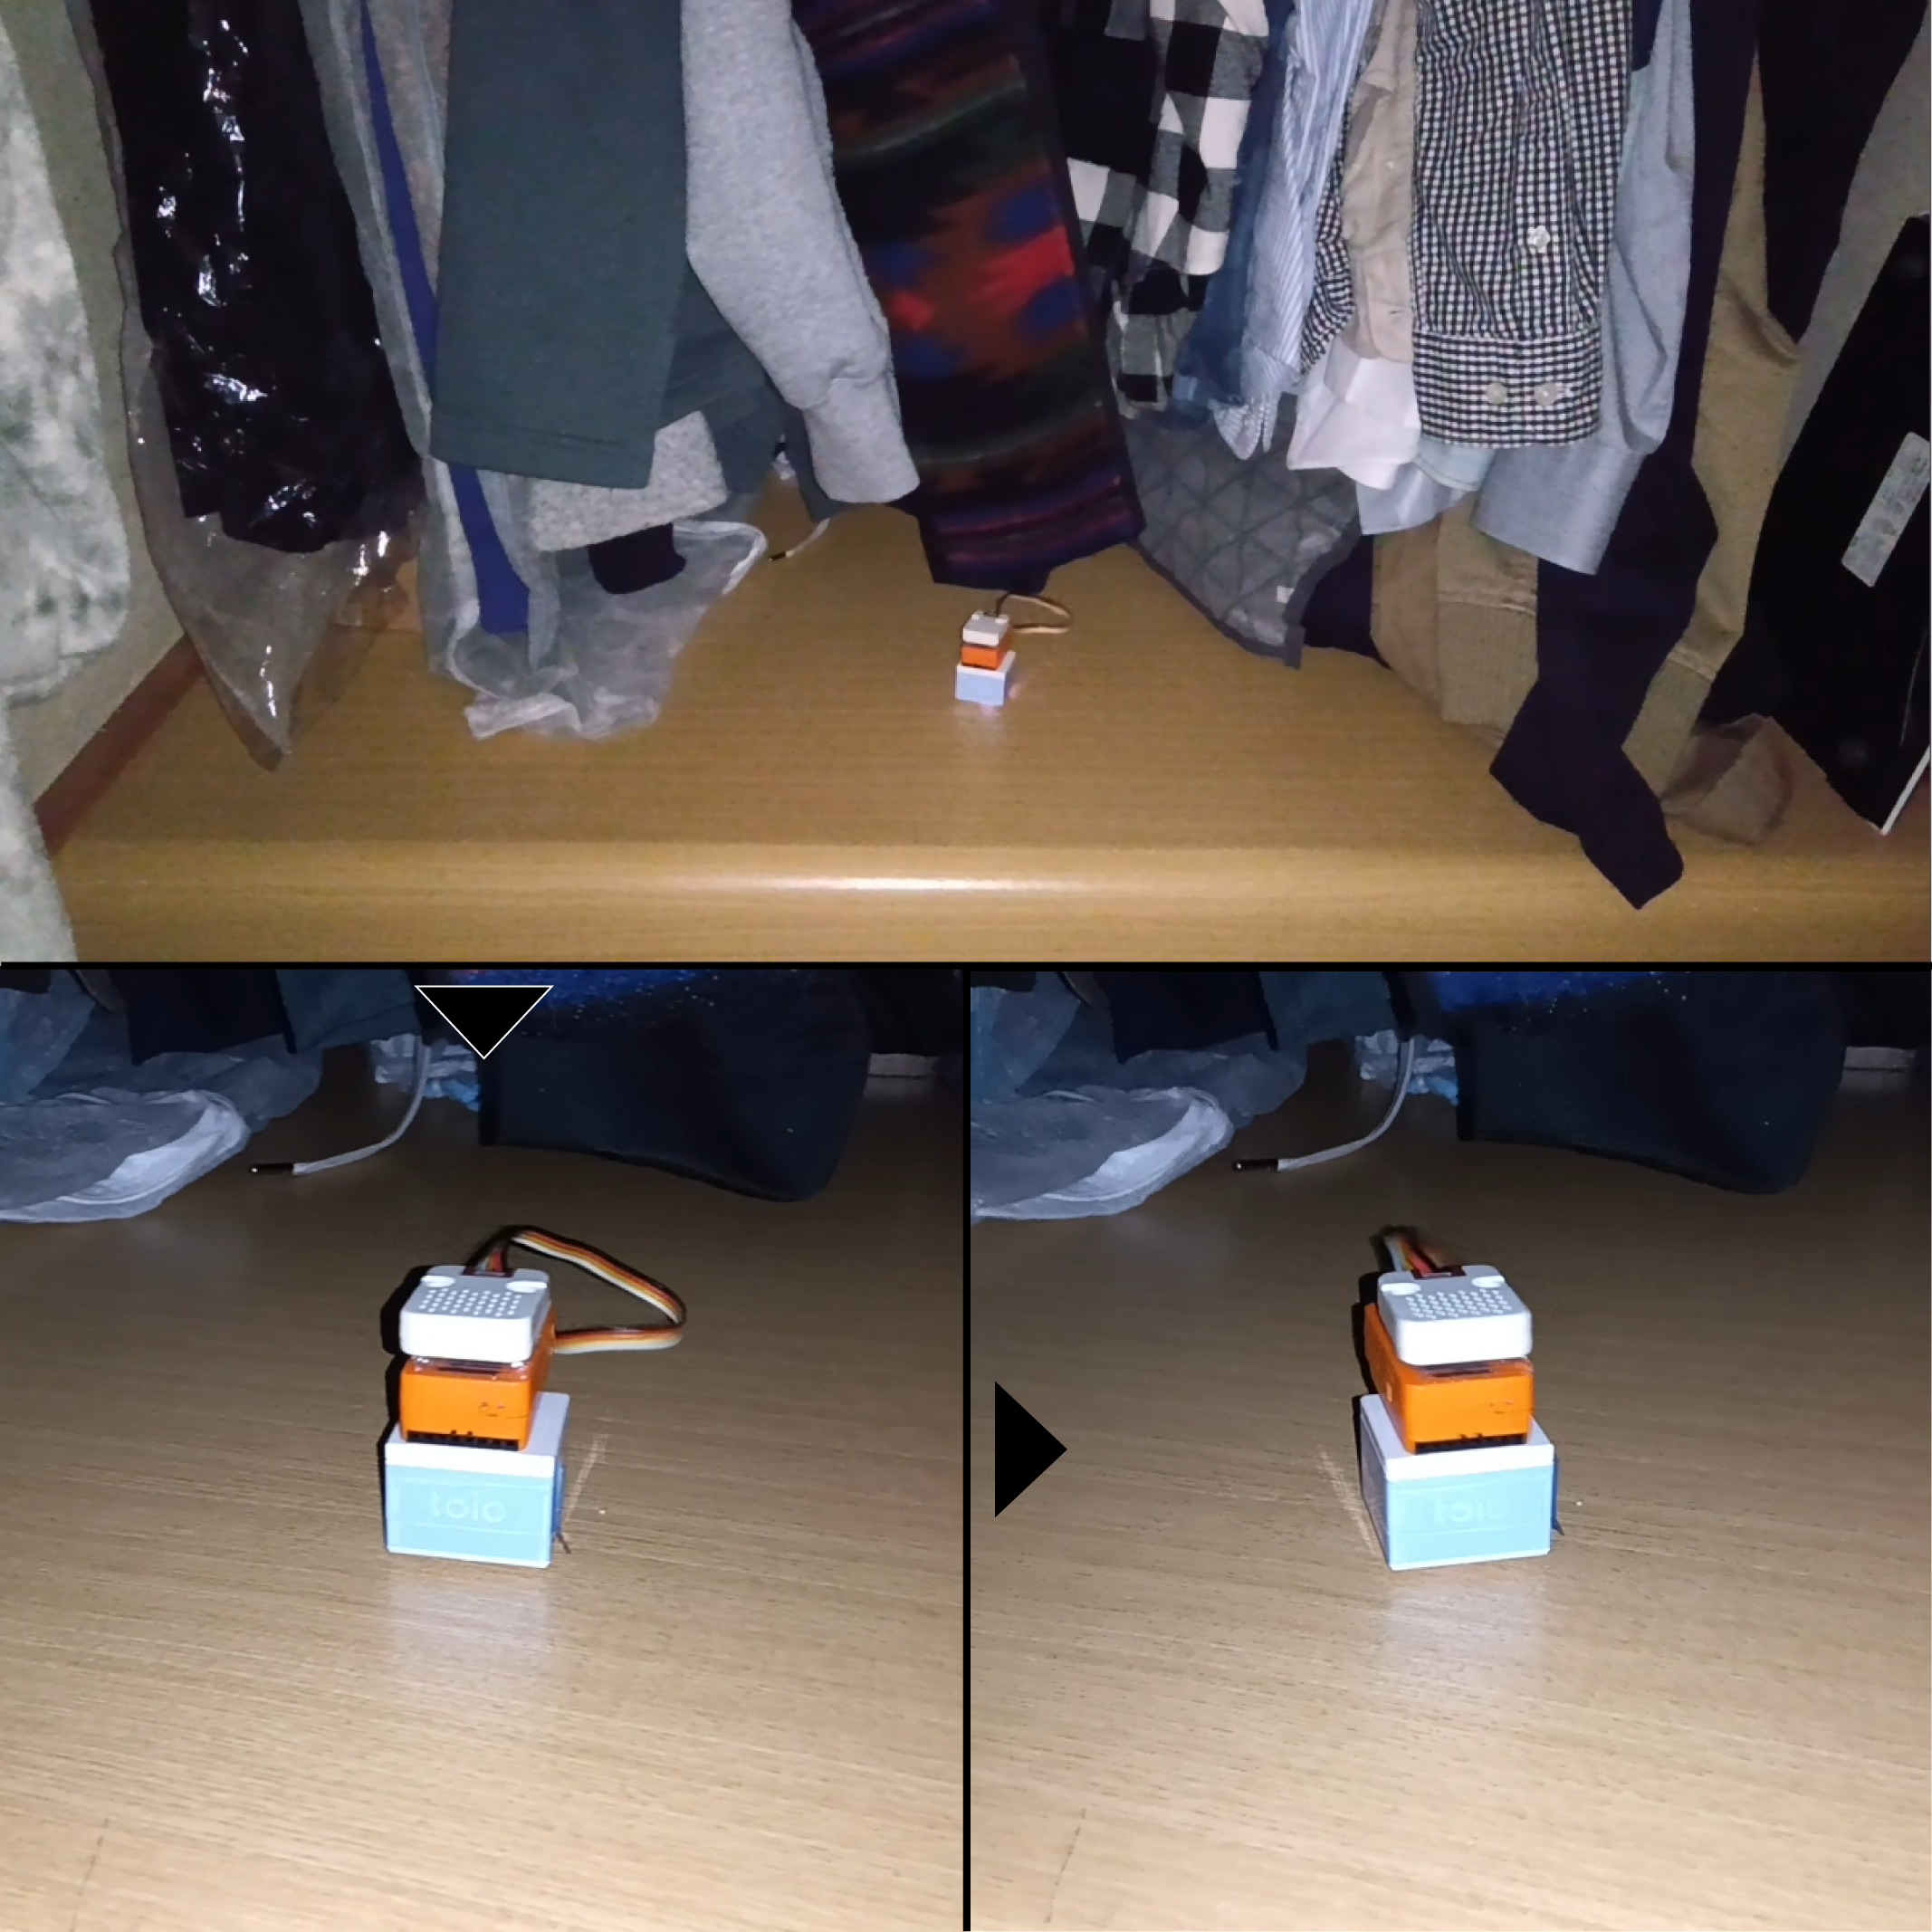
\includegraphics[keepaspectratio, scale=0.1]{resources/clothes.png}
      \caption{服の保存環境評価}
    \end{minipage}
    \label{fig:system-test}
  \end{center}
\end{figure*}

本研究では、生活空間において人間以外の存在と共存する中で、それぞれの環境評価を理解し合えるシステムの開発を行った。従来、環境の快・不快の評価は個人の感覚や基準で捉えられており、その感覚を直接共有することは困難であった。そこで、環境センサーを用いて取得したデータに基づき、人間、動植物、非生物などの環境評価基準を設定し、その評価結果をロボットの身体的動作を通じて表現するシステムを構築した。

\section*{システムの特徴}
開発したシステムは以下の3つの特徴を持つ:

\begin{enumerate}
  \item 継続的な表現:生活空間において、ロボットが常に存在し続けることで、環境変化に応じた他者の評価を途切れることなく表現できる。
  \item 多様な他者の表現:人間、動物、植物など様々な他者の環境評価基準を設定し、それぞれの特徴を反映した動作で表現できる。
  \item 自然な理解支援:ユーザーが特別な操作をすることなく、生活空間における他者との環境認識の違いを自然に理解できる。
\end{enumerate}

\section*{実装と検証}
システムは、センシング、評価、アクション生成、ロボット制御の4つのモジュールで構成されている。評価システムでは、温度・湿度などの環境データを取得し、対象ごとに設定された最適環境条件との差異をスコア化する。例えば、人間の場合は気温18〜24℃を快適範囲とし、この範囲から外れた場合はロボットが不安定な動きで表現する。

検証実験では、人間、猫、バナナ、衣服の4種を評価主体として実装を行った。それぞれの対象について特徴的な環境条件を設定し、条件からの逸脱度に応じてロボットの動作パターンを変化させることで、環境評価の違いを視覚的に表現することに成功した。

\section*{今後の展望}
本研究の成果により、生活空間における多様な存在との共生に向けた新しいインタラクションの可能性を示すことができた。今後は、より多様な環境要因の考慮や、センサー・ロボットの組み合わせによる表現の拡張を進めることで、ユーザーと他者との相互理解をさらに促進できると考えられる。

\end{document}
